%%%%%%%%%%%%%%%%%%%%%%%%%%%%%%%%%%%%%%%%%
% Masters/Doctoral Thesis 
% LaTeX Template
% Version 2.4 (22/11/16)
%
% This template has been downloaded from:
% http://www.LaTeXTemplates.com
%
% Version 2.x major modifications by:
% Vel (vel@latextemplates.com)
%
% This template is based on a template by:
% Steve Gunn (http://users.ecs.soton.ac.uk/srg/softwaretools/document/templates/)
% Sunil Patel (http://www.sunilpatel.co.uk/thesis-template/)
%
% Template license:
% CC BY-NC-SA 3.0 (http://creativecommons.org/licenses/by-nc-sa/3.0/)
%
%%%%%%%%%%%%%%%%%%%%%%%%%%%%%%%%%%%%%%%%%

%----------------------------------------------------------------------------------------
%	PACKAGES AND OTHER DOCUMENT CONFIGURATIONS
%----------------------------------------------------------------------------------------


\documentclass[
11pt, % The default document font size, options: 10pt, 11pt, 12pt
%oneside, % Two side (alternating margins) for binding by default, uncomment to switch to one side
english, % ngerman for German
singlespacing, % Single line spacing, alternatives: onehalfspacing or doublespacing
%draft, % Uncomment to enable draft mode (no pictures, no links, overfull hboxes indicated)
%nolistspacing, % If the document is onehalfspacing or doublespacing, uncomment this to set spacing in lists to single
%liststotoc, % Uncomment to add the list of figures/tables/etc to the table of contents
%toctotoc, % Uncomment to add the main table of contents to the table of contents
%parskip, % Uncomment to add space between paragraphs
%nohyperref, % Uncomment to not load the hyperref package
headsepline, % Uncomment to get a line under the header
%chapterinoneline, % Uncomment to place the chapter title next to the number on one line
%consistentlayout, % Uncomment to change the layout of the declaration, abstract and acknowledgements pages to match the default layout
]{MastersDoctoralThesis} % The class file specifying the document structure


\usepackage[utf8]{inputenc} % Required for inputting international characters
\usepackage[T1]{fontenc} % Output font encoding for international characters
\usepackage{palatino} % Use the Palatino font by default



\usepackage{pslatex}
\usepackage{graphicx}
\usepackage{wrapfig}
\usepackage[font={small,it}]{caption}
\usepackage{subcaption}
\usepackage{algorithm}
\usepackage{algpseudocode}
\usepackage{mathtools}
\usepackage{amsmath,amssymb}
\usepackage{float}
\usepackage[toc,page]{appendix}

\usepackage{tikz}
\usepackage{collcell}
\usepackage{xstring}
\usepackage{colortbl}
\usepackage{graphicx}
\usepackage{pdftexcmds}
\usepackage{textcomp}

\usepackage[
backend=biber,
sorting=ynt
]{biblatex}
\bibliography{references.bib}
\usepackage[autostyle=true]{csquotes} % Required to generate language-dependent quotes in the bibliography


%----------------------------------------------------------------------------------------
%	MARGIN SETTINGS
%----------------------------------------------------------------------------------------

\geometry{
	paper=a4paper, % Change to letterpaper for US letter
	inner=2.5cm, % Inner margin
	outer=3.8cm, % Outer margin
	bindingoffset=.5cm, % Binding offset
	top=1.5cm, % Top margin
	bottom=1.5cm, % Bottom margin
	%showframe, % Uncomment to show how the type block is set on the page
}

\newcommand\defeq{\stackrel{\mathclap{\small\mbox{def}}}{=}}
\newcommand\IE{\mathbb{E}}

\newcommand*{\MinNumber}{0}
\newcommand*{\MaxNumber}{20}


%----------------------------------------------------------------------------------------
%	THESIS INFORMATION
%----------------------------------------------------------------------------------------

\thesistitle{Exploring and Exploiting Monte-Carlo Othello} % Your thesis title, this is used in the title and abstract, print it elsewhere with \ttitle
\supervisor{dr. ir D. \textsc{Thierens}} % Your supervisor's name, this is used in the title page, print it elsewhere with \supname
\examiner{} % Your examiner's name, this is not currently used anywhere in the template, print it elsewhere with \examname
\degree{Bachelor of Science} % Your degree name, this is used in the title page and abstract, print it elsewhere with \degreename
\author{Richard \textsc{Deurwaarder}} % Your name, this is used in the title page and abstract, print it elsewhere with \authorname
\addresses{} % Your address, this is not currently used anywhere in the template, print it elsewhere with \addressname

\subject{Artificial Intelligence} % Your subject area, this is not currently used anywhere in the template, print it elsewhere with \subjectname
\keywords{Bandit problems, UCT, Monte carlo tree search, Othello} % Keywords for your thesis, this is not currently used anywhere in the template, print it elsewhere with \keywordnames
\university{Utrecht University} % Your university's name and URL, this is used in the title page and abstract, print it elsewhere with \univname
\department{} % Your department's name and URL, this is used in the title page and abstract, print it elsewhere with \deptname
\group{} % Your research group's name and URL, this is used in the title page, print it elsewhere with \groupname
\faculty{} % Your faculty's name and URL, this is used in the title page and abstract, print it elsewhere with \facname

\AtBeginDocument{
	\hypersetup{pdftitle={Exploring and Exploiting Monte-Carlo Othello}} % Set the PDF's title to your title
	\hypersetup{pdfauthor={Richard Deurwaarder}} % Set the PDF's author to your name
	\hypersetup{pdfkeywords={Bandit problems, UCT, Monte carlo tree search, Othello}} % Set the PDF's keywords to your keywords
	\hypersetup{%
		colorlinks = true,
		linkcolor  = black
	}
}

\begin{document}

%----------------------------------------------------------------------------------------
%	TITLE PAGE
%----------------------------------------------------------------------------------------

\begin{titlepage}
	\centering
	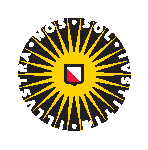
\includegraphics[width=0.20\textwidth]{images/uu-logo}\par\vspace{1cm}
	{\scshape\LARGE Utrecht University \par}
	\vspace{0.5cm}
	{\scshape\Large Artificial Intelligence\par}
	{\scshape\Large Bachelor Thesis (15 ECTS)\par}
	\vspace{1.5cm}
	{\huge\bfseries Exploring and Exploiting Monte-Carlo Othello\par}
	\vspace{0.5cm}
	{\Large\itshape Richard Deurwaarder\par}
	\vfill
	supervised by\par
	dr. ir. D. \textsc{Thierens}
	
	\vfill
	
	% Bottom of the page
	{\large \today\par}
\end{titlepage}

\tableofcontents % Prints the main table of contents

%----------------------------------------------------------------------------------------
%	THESIS CONTENT - CHAPTERS
%----------------------------------------------------------------------------------------


\mainmatter % Begin numeric (1,2,3...) page numbering

\pagestyle{thesis} % Return the page headers back to the "thesis" style

\chapter{Introduction}

\section{Overview}
Monte Carlo planning has long been a good solution to find near-optimal solutions to large state space Markovian Decision Problems (MDP). This is a type of problem where an action needs to be taken which partly influences what new state is reached. Each state can be associated with a reward, this reward needs to be optimized. When the problems become sufficiently large it quickly becomes infeasible to search the whole state-space and trade-offs need to be made. In this thesis, I will look at the board game Othello, find good moves for Othello can be described as an MDP and its state space is far too large to search through.\\

In problems with such large state spaces, it is useful to gather information about which actions are more promising than others and put more effort into investigating states resulting from those promising actions. Gathering information costs time and is not directly useful for our solution, ideally we want to spend just enough time gathering information to identify the good actions and focus investigating which action is best. This is the classic exploration versus exploitation problem: How much effort do we put into exploring how promising the actions are and how much effort is put into exploiting this information. One algorithm proposed by Kocsis and Szepesvari\cite{Kocsis:2006} called UCT deals with this problem.\\

UCT uses an algorithm called Monte Carlo Tree Search in combination with a (modified)  selection policy called UCB1. UCT introduces a parameter sometimes called the exploration parameter usually denoted by c or $C_p$. This c-value drives how much exploring and exploiting is done. In practice, this parameter is chosen without too much consideration.\\

\section{Research questions}
\label{section:research-questions}
The main question I will answer is how important it is to pick a good $c$-value when using the UCT algorithm. To answer this question, experiments will show if using different $c$-values impacts the quality of the solutions provided by UCT. By using Othello as a specific problem I can test if any optimal c-values exist with respect to other $c$-values and lastly when comparing optimal $c$-values with suboptimal values I can measure the actual impact of choosing suboptimal $c$-values.\\

The main question: How important is it to pick an appropriate $c$-value when using UCT.

Will be answered by providing insight in the following research questions:
\begin{itemize}
	\item How do different $c$-values in UCT compare?
	\item Is there any optimal $c$-value for a given problem?
	\item Is there a significant difference when using the optimal $c$-value versus other $c$-values?
\end{itemize}
\section{Structure}
To answer these questions I will provide the context in which the experiments will be run. Starting off explaining the Exploration versus Exploitation in more detail and introducing a metric called regret which measures how much effort is wasted on exploring suboptimal actions.\\ This is followed by an in-depth explanation of game Othello and the Monte Carlo Tree Search algorithm. This will show how the algorithm can be used to search for good Othello moves and why Othello moves are a good problem to analyze MCTS with. This is partly because Othello is a two player game Othello, this gives us a very natural way of comparing different c values by just letting them play games against each other.\\
I will explain exactly how I have set up each test and discuss the results. TODO


\chapter{Problem analysis}

\section{Exploration vs Exploitation}
At the heart of Monte Carlo planning algorithms lies the Exploration versus Exploitation dilemma. The Multi Arm Bandit problem is a classic approach to demonstrate this dilemma and introduces a metric called regret. Regret can be used to define how much time has been spent exploring suboptimal possible solutions. Using the bandit problem we can reason about what information regret actually gives us and show some of the theoretical limits for regret while searching for a solution.

\subsection{Multi-Arm Bandit Problem}
The multi-arm bandit problem can be described as follows: Imagine multiple slot machines in a casino, each having an arm to initiate actually playing the machine. Playing a machine will give some sort of reward or payout. Which while random does follow some sort of distribution. The objective is to maximize the sum of the rewards earned through a sequence of machines played.\\

Formally we can define a K-armed bandit problem by random variables $X_{i,n}$ for $1 \leq i \leq K$ where each $i$ is the index of a machine and $K$ the number of machines. Successive plays of machine $i$ yield rewards $X_{i,1},X_{i,2},X_{i,3}...$ which are independent, identically distributed and have an unknown expected value of $\mu_i$.

\subsection{Regret}
Regret is defined as the amount of reward we did not receive because the optimal machine was not chosen. For example, because we were exploring other arms. Let $\mu_i$ be the expected reward for machine $i$ and $\mu^{*} \defeq \max\limits_{1 \leq i \leq K} (\mu_i)$ or in words $\mu^{*}$ the expected reward of the optimal machine. $n$ the total amount of plays. $T_i(n)$ the number of times machine $i$ has been played at $n$ plays. $\IE[*]$ is used to denote expectation. Then the total regret can be defined as:
\[
    regret = \mu^*n - \sum_{i=1}^{k}\mu_i\IE[T_i(n)]
\]
or in words: the expected value of the best arm times $n$, minus expected value of each arm times the number of times that arm has been played.\\

Extensive analysis has been done on this subject. A lower bound for regret has been found in 1985 by Lai and Robbins\cite{Lai+Robbins:1985}. They showed, for a wide variety of reward distributions, a logarithmic increasing regret is the best any policy can do. 

\begin{figure}
	\centering
	\begin{subfigure}{0.4\textwidth}
		\caption{Start position}
		\label{fig:othello-startposition}
		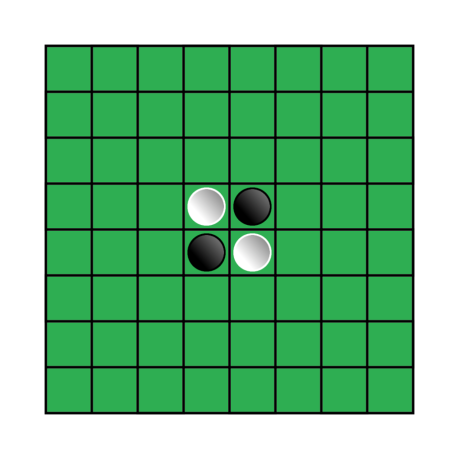
\includegraphics[width=\textwidth]{images/startposition}
	\end{subfigure}%
	\begin{subfigure}{.4\textwidth}
		\caption{White captures}
		\label{fig:othello-capture}
		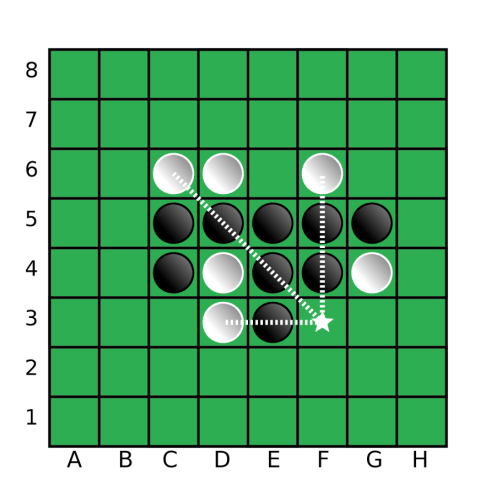
\includegraphics[width=\textwidth]{images/capture}
	\end{subfigure}
	\caption{Uncheckered 8x8 boards}
\end{figure}
\begin{figure}[H]
	\centering
	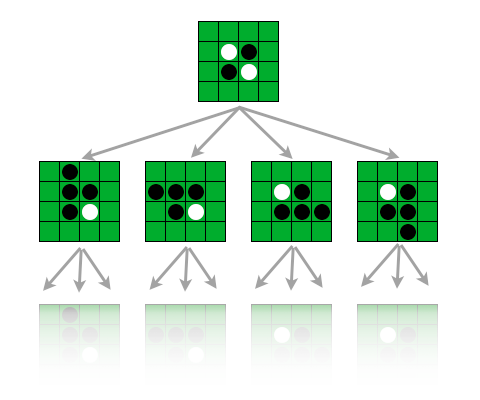
\includegraphics[width=0.4\textwidth]{images/othello-gametree}
	\caption{Othello tree representation}
	\label{fig:othello-gametree}
\end{figure}
\section{Othello}
Othello is a strategy board game for two players. Sometimes also referred to as Reversi. The Exploration vs. Exploitation dilemma presents itself in the game Othello when deciding what move to make. This happens when a player has multiple valid moves, figure \ref{fig:othello-gametree}) shows 4 possible moves when starting at figure \ref{fig:othello-startposition}. The different moves can be seen as different `arms' in the Multi Armed Bandit problem.\\
Othello players are assigned a color and take turns placing pieces on the board while capturing pieces of the other player. The player with most pieces left at the end of the game wins.
\subsection{Terminology}
These are the terms used when referring to the different components and concepts of the Othello game:
\begin{itemize}
	\item Color, each player gets assigned a color, black or white.
	\item Piece, each player makes moves by placing a piece\footnote{Sometimes referred to as a disk} of their own color on the board.
	\item Move, a move consists of adding one piece to the board.
	\item Squares, a square is a possible position for a piece to be or have been placed on. 
	\item Board, the board is where all moves are being made on, it consists of 8 by 8 squares on which to put our pieces on. Pieces can not be placed on multiple squares or by overlapping any edges, see fig \ref{fig:othello-startposition} for correctly placed pieces.
	\item Corner move, a corner move is a move where you place a piece on one of the four corners of the board.

\end{itemize}
\subsection{Board and moves}
Othello is played on a board of 8 by 8 squares\footnote{Versions of Othello are sometimes played with bigger boards, in this thesis I will only consider 8x8 boards.}. It always has the same starting position as shown in figure \ref{fig:othello-startposition}. A move is done by placing a piece on an empty square and capturing at least one piece of the opponent in the process. A piece is captured when it becomes surrounded by the other color, see figure: \ref{fig:othello-capture}. When white places a piece on F3. Five pieces get captured and turn white. Because every move must capture at least one opponent's piece, this greatly limits the number of possible moves. Sometimes no valid moves are possible, when this happens the turn is skipped and the opponent can go again.
\subsection{Game results} The winner of the game is determined by the player with the most pieces at the end of the game. The game ends is when no other available moves are left, this might happen before all the squares are filled, because you may only place a piece if you capture at least one other. It does not matter by how many pieces you beat the opponent.
\subsection{Importance of different squares} The pieces in the middle of the board might be captured and recaptured multiple times because they are surrounded by so many different positions but the corner squares will never be captured once initially filled, because they cannot be surrounded, making it a safe and valuable position to take. We would expect an algorithm to take advantage of this. By proxy, this makes placing a piece on one of the 3 squares surrounding a corner a bad move, because this allows the opponent to make a corner move.

\subsection{Exploring and exploiting with Othello}
Monte Carlo tree search, and especially UCT, has been tested and analyzed using board games such as Othello, Chess, Go etc. Most notably with Go, a lot of progress has been made recently, where MCTS has been used in combination with Deep neural networks beating (human) world champions\cite{deepmind}.\\
The reason these board games work well when analyzing is because they have no hidden information. The algorithm can see exactly where all the pieces are on the board and requires no context or historic moves to decide what move it is going to make. Games where not all information is shared among the players are games such as poker or blackjack, each player only knows it's own cards.\\

In this thesis, I will test and compare specific values of the exploration parameter (c-value) against other c-values. Two player games provide a very naturally means of comparing these two values by just playing them against each other and see who wins the game.\\
Othello, in particular, makes a good test-case because the game length has a hard limit. Once the board is full the game is over, this limits the game to a maximum of 60 moves. The possible amount of valid moves per turn is generally small, staying under 8-10 generally. Having smaller and thus computationally faster games allows for less noise in the results because we can test more games.

\section{Monte Carlo Tree search}
Using Monte Carlo Tree search(MCTS) in combination with Othello we are presented with a clean instance of the Exploration versus Exploitation dilemma. MCTS searches through a (game)tree structure and gathers information by sampling the tree lots of times. An Othello turn with all the possible moves that are available to the player can be represented by such a tree structure.\\ MCTS works by selecting a move and simulates games using this move as a start. By taking many samples the algorithm gets information on how well certain moves perform, performing could be defined by how many games have been won when simulating using a certain move.  Using a minimax tree it is possible to represent the opponent's moves too in an Othello game, where a player would like to maximize its own score and at the same time minimize their opponent's score. 
Exploration vs exploitation presents itself when we need to make a decision for what Othello move we are going to use to simulate games. Will we choose the best move so far? Or are we going to try other moves to see if they have potential.

\subsection{Tree search}
The possible moves of a turn and their subsequent possible moves can be represented as a tree structure, see figure \ref{fig:othello-gametree} for such a tree without the subsequent moves, figure \ref{fig:mcts-gametree-values} with subsequent moves but without the image of the board per node. The root of the tree is the current state of the board. Edges represent (valid) moves, nodes represent a state of the board. Leafs (a node without any children) represents the state of the board of a finished game. A path from the root node to a leaf shows us a way the game could be played. Tree structures like these can be called game trees. Searching through these game trees and finding an optimal or nearly optimal move to make can be achieved via different algorithms. The size of the tree is an important indicator of how complex a game is for an algorithm to handle. This is usually described by a depth and branching factor. In Othello the depth of a tree is limited, it can not be any bigger than 60, because only one piece is played per move and there are 60 empty squares. Not every game ends with a full board the average amount of moves and thus the depth of the tree is around 58. The branching factor is estimated to be around 10 according to L. Allis\cite{Allis:1994}.

\begin{figure}[t]
	\centering
	\begin{subfigure}{0.3\textwidth}
		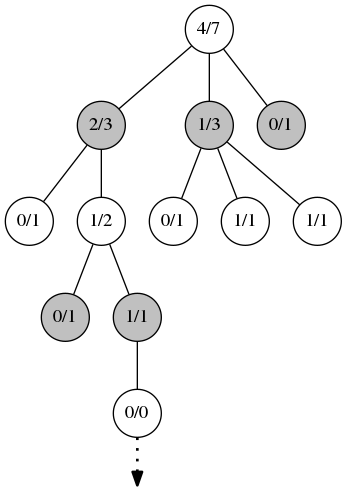
\includegraphics[width=\textwidth]{images/gametree-values}
		\caption{Game tree with values.}
		\label{fig:mcts-gametree-values} 	
	\end{subfigure}%
	\unskip\ \vrule\
	\begin{subfigure}{0.3\textwidth}
		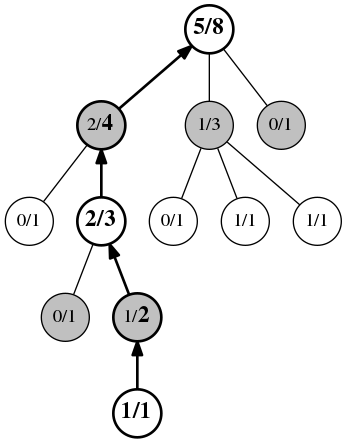
\includegraphics[width=\textwidth]{images/gametree-values-updated}
		\caption{Game tree with updated values after a win.}
		\label{fig:mcts-gametree-values-updated}
	\end{subfigure}
	\caption{MCTS Minimax game tree}
\end{figure}

\subsection{Minimax tree}
Minimax is a way to search through a game tree and find a good action in a turn-based game such as Othello. With a plain game tree, you might store win percentages for each node. In a minimax tree, you would slightly alter this and take into account for what player you are computing the tree. For a minimax tree to compute white's best move, nodes, where it is the white player's move, would still have the win percentage, however for the nodes where it is black's turn you would actually store the loss rate of the white player. Figure \ref{fig:mcts-gametree-values} shows a game tree with values per node. The values for each node indicate how well this node is for the players. White will choose actions that will maximize it's own score, while black will choose actions that minimize the score of white.

\begin{algorithm}
\caption{Monte Carlo Tree Search}
\label{algo:mcts}
\begin{algorithmic}
\Function{MonteCarloPlanning}{rootNode}
\While{no timeout}
\State $leafNode \gets \Call{Select}{rootNode}$
\State $(action, newNode) \gets \Call{Expand}{leafNode}$
\State $reward \gets \Call{Simulate}{newNode}$
\State $ancestors \gets \Call{getAncestors}{newNode}$
\State \Return \Call{UpdateValue}{ancestors}
\EndWhile
\State \Return \Call{bestAction}{state, 0}
\EndFunction
\end{algorithmic}
\end{algorithm}
\subsection{Algorithm}
Because there are many possible board states, the game tree would be far too large to generate completely. Instead of generating the whole tree, MCTS uses simulations to direct what parts of the tree to generate. These simulation steps will very quickly and in usually a stochastic manner `finish' the remainder of the game steps, for instance by making random moves until the game ends. This simulation gives an idea how well the nodes perform. In essence, the simulation is sampling from all possible games that could happen for the node in question. The evaluation of this simulation will be used to update the parent nodes in the tree, which in turn is used to decide what node will be added next and used for the next simulation. This is the basic idea behind Monte Carlo Tree Search (MCTS).

MCTS (algorithm \ref{algo:mcts} for pseudo code) can be split up into four parts:
\begin{enumerate}
    \item SELECT, in this step the algorithm will find a node with an action that has not been investigated yet.
    \item EXPAND, using the node and an action that has not been investigated this step will expand the tree and add a new node.
    \item SIMULATE, Using the new node this step will perform a (fast) simulation of how the game might finish from that point n. For example by taking random actions until the game is over. Note that states generated in the simulation will not be stored or added to the tree. We're only interested in the final evaluation, has player 1 won or lost. This is also the place to insert domain knowledge about the problem. Rather than making random moves, some fast heuristic might be used to generate more realistic simulations.
    \item UPDATEVALUE, updating the values for each node is important to actually make the final decision as to which action we will take. Figure \ref{fig:mcts-gametree-values} shows an example game tree. The numbers indicate how many simulations resulted in a player 1 win and how many have been simulated in. Figure \ref{fig:mcts-gametree-values-updated} shows we update each node. 
\end{enumerate}

\section{UCT}
UCT has been introduced by L. Kocsis and C. Szepesv{\'a}ri in 2006\cite{Kocsis:2006}. UCT drives the selection of nodes in the first step of MCTS. UCT is short for UCB applied to trees, meaning it is a modification of the UCB policy to allow for tree searching. UCB stands for Upper Confidence Bounds.
\subsection{UCB}
UCB has been introduced by P. Auer, N. Cesa-Bianchi and P. Fischer in Finite-time analysis of the Multiarmed Bandit problem\cite{auer2002finite}. UCB is a policy for selecting the next action to try. It does this by determining the value called Upper confidence bound for each possible action. This upper confidence bound is an optimistic estimate of the true expected reward for an action, optimistic indicating it would rather estimate higher than lower, but still be realistic given the rewards returned thus far.\\
The reason it would rather be too high than too low has to do with what it's trying to minimize: the regret. Note regret is the amount of reward we are missing because we did not try the best possible action. So by always choosing the action with the highest reasonable reward, the expectation is we will be getting a high reward.\\
In the context of MCTS, the UCB policy determines what action will be selected to run the simulation on. It does this based on how many times an action has been chosen and the amount of reward that has been gathered.\\

UCB1 starts off by playing each action once. Each next action is chosen by picking the action which maximizes:
\[
    x_j + \sqrt{\dfrac{2 lg(n)}{n_j}}
\]

\textit{$x_j$ is the average reward for the action, $n_j$ is the number of times the action has been played and n is the total number of plays so far.\\}

The reason this works so well is because is shown by in \cite{auer2002finite} by P. Auer et al. They have proved when using this selection policy, the expected cumulative regret is at most: 
\[
    \Bigg[ 8 \sum_{i:\mu_i\lneq\mu^*}\bigg(\dfrac{ln(n)}{\Delta_i}\bigg)\Bigg] + \Bigg( 1 + \dfrac{\pi^2}{3}\Bigg)
    \Bigg(\sum_{j=1}^{k}\Delta_j\Bigg)
\]

\textit{$\Delta_j$ is defined as the difference between the expected reward of $j$ and the maximum reward possible.\\}

This bounds the regret to be logarithmically in terms of $n$ plays. Furthermore, this is not only a bound on the regret asymptotically but actually for any number $n$ plays.

\subsection{UCB for tree search}
UCB1 has a good bound on the regret and works well in bandit-like problems but UCB1 is not designed to be used in a tree search. UCT modifies this slightly. The basic idea proposed by L. Kocsis and C. Szepesv{\'a}ri in Bandit based Monte-Carlo Planning\cite{Kocsis:2006} is to use the UCB1 in a recursive manner.\\

Remember this is only used to select the node that MCTS will use for simulation:

Let the current node be the root node of the tree.
\begin{enumerate}
	\item if the current node has any un-played child, return this node to MCTS.
	\item if every child has at least 1 play, set the current node to the child node that maximizes:
	\[
	x_j + 2c\sqrt{\dfrac{ln(n)}{n_j}}
	\]
	\item Loop step one and two until an unplayed child has been found.
\end{enumerate}


The formula in step two is slightly different than the formula used in UCB1, most notably the introduction of the c-value. This c-value is where we will be looking at in the experiments.\\

When the c-value rises, the policy will put more emphasis on how confident we are about the reward so far ($x_j$). Or in order words the higher the c-value gets, the more often we will be exploring other actions.

\chapter{Experiment details}
To run the experiments I implemented Monte Carlo Tree Search as described in the MCTS and UCT sections. However, some specific decisions regarding the implementation of the algorithms and how to run the experiments had to be made.

\begin{figure}[h]
	\centering
	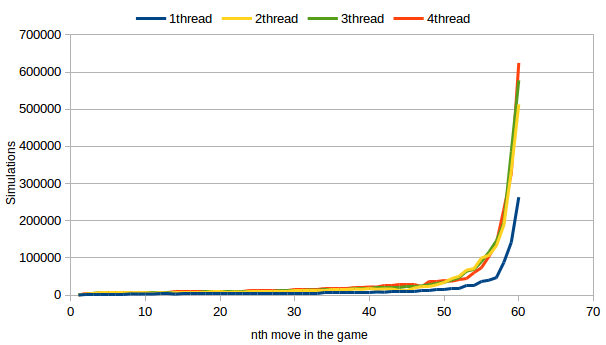
\includegraphics[width=0.5\textwidth]{images/mcts-simulations-threads}
	\caption{The number of simulation runs per move. Data has been shown for 1,2,3 and 4 threads, using random simulations.}
	\label{fig:mcts-threads}
\end{figure}

\section{Parallel MCTS}

The MCTS algorithm has been slightly adjusted to take advantage of multiple CPU cores by running the algorithm with multiple threads.\\

Using multiple threads increases the number simulation runs per second significantly as shown in figure \ref{fig:mcts-threads}. It shows going from one thread to two threads increases the number of simulations done by a factor of 2 or 3. Using three and four threads gives a very small increase in simulations done. More than four threads has been tested but does not show any increase in performance (as expected with 4 CPUs). Because of this the choice has been made to run all tests with four separate threads, although the biggest boost in the number of simulations happened at two threads there's no disadvantage in using four threads.\\

The algorithm has been adjusted as described in the paper Parallel Monte-Carlo Tree Search\cite{chaslot2008parallel} by Guillaume et al. Locking per node has been implemented, meaning when adding a new node to the game tree or when updating values in the game tree the node in question is locked, rather than locking the whole tree.

\begin{figure}
	\centering
	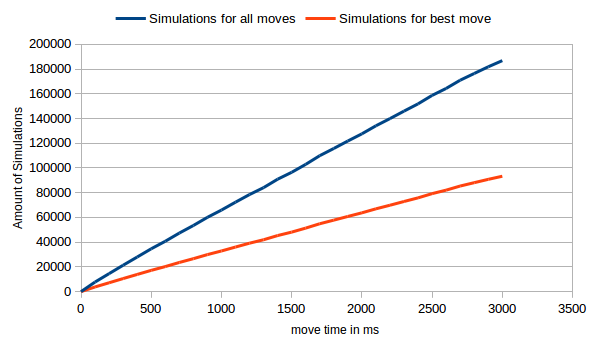
\includegraphics[width=0.5\textwidth]{images/simulations-time}
	\caption{The number of simulation runs per move. For different amounts of time per move. Blue is the total amount of simulations made. Orange is the number of simulation runs for only the best (corner) move.}
	\label{fig:mcts-simulations-time}
\end{figure}

\section{Move \& game runtimes}
Because MCTS effectively samples a large state space, it does not terminate at any particular point. A decision has to be made how much time can be spent per move and thus per game.\\

Figure \ref{fig:mcts-simulations-time} shows the number of simulations when we increase the time per move from 100ms to 3000ms. It shows a very linear relationship, both in total simulations as simulations for what it considers the best move. This indicates there is no particular threshold or specific value which would give a better performance-per-second spend.\\

I have decided on 500ms per move. An Othello game consists of maximally 60 moves. At 500ms per move, this comes down to roughly 30 seconds per game. There is some overhead between the moves, but this is largely compensated by the fact that not every game has exactly 60 moves, the average of moves per game is closer to 57-58 moves.\\

The 500ms is CPU time per thread, with 4 threads this comes down to 2000ms of CPU time total. Figure \ref{fig:mcts-threads} shows the number of simulation runs per move increases as the game progresses. This happens because each simulation takes less time depending on how many moves are left in the game\footnote{Simulations on a board with only one empty square finish a lot faster than having to play out a game with 40 empty squares.}. On average this comes down to 20.000 simulations per move if we do not take into account the big spike at the final few moves\footnote{With the big spike, it would go up to about 40.000 simulation runs.}.\\

\begin{figure}
	\centering
	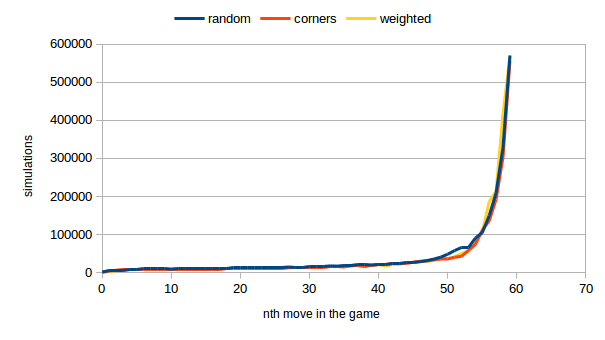
\includegraphics[width=0.5\textwidth]{images/mcts-simulations-domainknowledge}
	\caption{The number of simulation runs per move. Data has been shown for random simulation, corners-first, weighted simulation. MCTS uses 4 threads.}
	\label{fig:mcts-domainknowledge}
\end{figure}

\section{Domain knowledge in simulation}
The simulation step of MCTS has been tested with 3 separate versions. When referring to these types of simulations I will call them random, corners and weighted.

\subsection{Random playout}
The first version is without any domain knowledge, the algorithm will simulate the game by making completely random moves.

\subsection{Corners first playout}
The second variety is the same as the first by making random moves, except when a corner move is available. If a corner move is available it will always make that move. The reasoning behind this is that corner moves are generally always a good move to make in Othello.

\subsection{Weighted playout}
The final version chooses what moves to make by using a matrix of weights. Each weight corresponding to a square on the Othello board. For instance choosing a corner will have a higher weight than choosing a square in the middle of the board. These weights are normalized per turn for all valid moves and give a probability for each possible move in that turn. See table \ref{table:othello-weights} in the appendix for the weights used. These weights have been calculated by P. Hingston and M. Masek in their paper Experiments with Monte Carlo Othello\cite{hingston2007experiments}. They used an Evolutionary strategy to find good values which they tested against several other algorithms.

\section{Types of experiments}
\label{section:type-experiments}
Three types of experiments have been run. Unless otherwise specified all experiments have been run with 500ms time per move, 4 threads and random simulations.

\subsection{Ranking}
\label{section:ranking}
The first, which I will call \textit{ranking}. This experiment determines differences between multiple c-values and allows us to rank them best to worse.\\

It consists of a population of c-values. Each c-value $c$ will play 10 games versus all the other c-values, $c$ makes the starting move in these 10 games. The reverse also happens, so each other c-values will each play 10 games versus $c$ where $c$ does not get the starting move. This gives the following total number of plays for c:
\[
   10 * (n-1) * 2
\]

With the total amount of games played at: 
\[
   n * (10 * (n-1))
\]

\textit{Where $n$ is the number of c-values in the population. The $n-1$ is because c-values will not play against themselves.}\\

For example: when the population of c values consists of 12 elements, at 500ms per move or 30s per game. The total time is roughly: $30s * (12 * 10 * (12-1) * 2) =  79200s = 22 hours$.

\subsection{1 versus 1 game}
The second type of test is to determine differences between two specific players. This experiment runs a number of games, ranging from 10 to 300 games, between two players. These 2 players generally only differ by one parameter, such as c-value, or time per move.
\subsection{Single move analysis}
The other experiment is about analyzing a single move. This is run on the board shown in figure \ref{fig:othello-corner-board} with it being black's turn. This is a board with 8 possible moves and one move being particularly good. The corner move (0,0) is a lot better than all the others because if black does not take it, white can in the next move. This corner allows for a very good position on the top row and consequently the right columns.\\

This makes for an interesting move to analyze.


\begin{figure}
	\centering
	\includegraphics[width=0.5\textwidth]{images/othello-beginner-bias}
	\caption{Testing a beginner bias for Othello. Accumulated win chance for the starting player during the 75 games played.}
	\label{fig:othello-beginner-bias}
\end{figure}
\section{Beginner bias}
For some games a beginner bias exists. This means the player starting has some slight advantage in winning games. If this is the case for Othello we would have to compensate for this, for example by multiple games instead of one, so both players start equal number of times.\\

To test for this bias I have let two identical players with c-value of 0.5 play 30 games against each other. Should no bias exist we should expect a win percentage close to 50\%. Figure \ref{fig:othello-beginner-bias} shows how to win chance changes during those 75 games. And indeed it shows the win percentage of white converges towards 50\%.


\chapter{Results \& Discussion}

Several experiments have been run in order to provide insight and possible answers to the research questions stated in section \ref{section:research-questions}. In this section I will provide and analyze the data of these experiments while also discussing what these results might imply.

\begin{figure}[th]
	\captionsetup{width=.45\textwidth}
	\begin{minipage}[t]{0.5\textwidth}
	    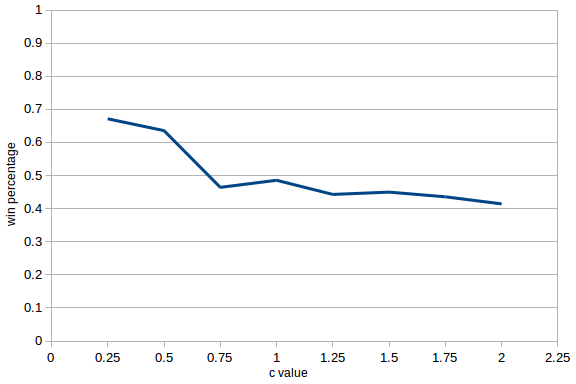
\includegraphics[width=\textwidth]{images/rank-raw}
	    \captionof{figure}{Results of having 8 c-values compete against each other. Data in appendix table \ref{table:results-rank-raw}.}
	    \label{fig:results-rank-raw}
	\end{minipage}%
	\begin{minipage}[t]{0.5\textwidth}
		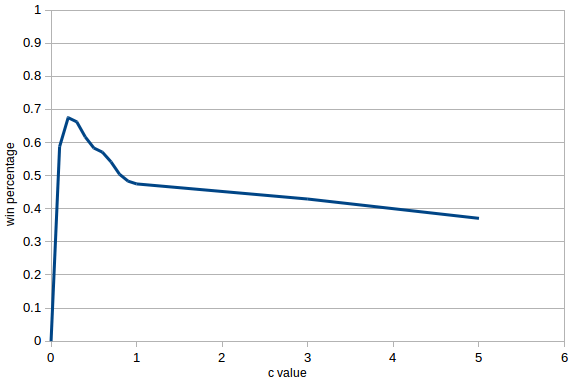
\includegraphics[width=\textwidth]{images/rank-015}
		\captionof{figure}{Results of having 13 c-values compete against each other. Data in appendix table: \ref{table:ranking-matrix-random}}
		\label{fig:results-rank-015}
	\end{minipage}
\end{figure}

\section{Is there a significant difference between c-values}
A pool of 8 distinct values has been tested using the ranking experiment (see section \ref{section:ranking}), the pool consisted of c-values: \{0.25, 0.5, 0.75, 1, 1.25, 1.5, 1.75, 2\}. Each value played 20 games against each of the other c-values in the pool. A total of 560 games have been played amongst them, where each single c-value played 140 games. The results are combined to form a win percentage per c-value in figure \ref{fig:results-rank-raw}. They show a decline in wins the higher the values get. This seems to indicate some sort of global maximum around the 0.25-0.5 interval.

\begin{figure}[t]
	\captionsetup{width=.45\textwidth}
	\begin{minipage}[t]{0.5\textwidth}
		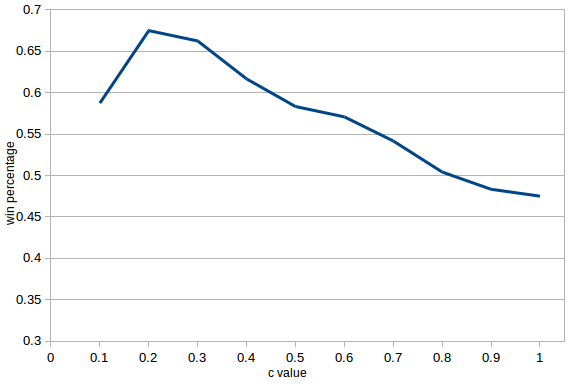
\includegraphics[width=\textwidth]{images/rank-01}
		\caption{The same values as figure \ref{fig:results-rank-015}, except with the c-values 0, 3 and 5 omitted and the y-axis cropped to the 0.3 to 0.7 range.}
		\label{fig:results-rank-01}
	\end{minipage}
	\begin{minipage}[t]{0.5\textwidth}
		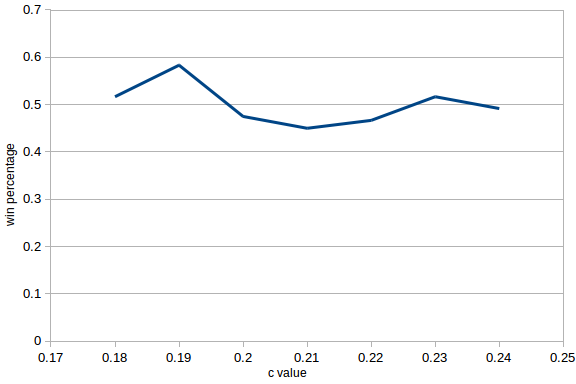
\includegraphics[width=\textwidth]{images/rank-narrow}
		\caption{Results of having 5 c-values compete against each other. Data in appendix table: \ref{table:ranking-matrix-random-narrow}.}
		\label{fig:results-rank-narrow}
	\end{minipage}
\end{figure}

\section{Higher resolution search for optimal c-values}
To narrow down on the insight from the previous test, another ranking test has been run with values closer to the best performing values of that previous test. These values are chosen around the 0.25-0.5 interval, the pool consisted of 13 c-values: \{0, 0.1, 0.2, 0.3, 0.4, 0.5, 0.6, 0.7, 0.8, 0.9, 1, 3, 5\}. Values 3 and 5 have been added to confirm there is not a local maximum for these values and give some context to the results we're seeing.\\

The results have been combined again in figure \ref{fig:results-rank-015}. They show the high c-values decline in win percentage the higher it gets as expected. This trend continus all the way to the 3 and 5 values adding more confidence to the claim that we are not dealing with a local maximum. An interesting result shows at a c-value of 0, the win percentage drops to nearly $0\%$.
Figure \ref{fig:results-rank-01} shows the same data but with a better resolution because the 0, 3 and 5 c-values have been omitted. It shows an increase in win percentage in the 0.1 to 0.2 range and a decline in the 0.2 to 1.0 range.\\

Zooming in even further using a new ranking experiment, figure \ref{fig:results-rank-narrow} shows the result of having a pool of c-values: \{0.18, 0.19, 0.20, 0.21, 0.22,0.23,0.24\} compete. For values in the 0.18 and 0.24 range win percentages start becoming more erratic and no real downwards slope is present. This seems to indicate the difference between values has become small enough to provide no further benefit.

Note that finding these optimal or very good performing c-values takes quite a bit of time. The time spend on these 4 tests adds up to about 48 hours. It is good to remember this as in certain use-cases it might not be worth spending this much time, when it is also possible to simply increase the time per move to compensate.


\vfill
\pagebreak
\begin{figure}[h]
	\captionsetup{width=.45\textwidth}
	\begin{minipage}[t]{0.5\textwidth}
		\centering
		\includegraphics[width=\textwidth]{images/ranking-118-124}
		\caption{Results of 4 c-values focused in the $[1.18,1,24]$ interval. Data can be found in appendix table \ref{table:ranking-matrix-random-narrow2}.}
		\label{fig:results-rank-0-01}
	\end{minipage}
	\begin{minipage}[t]{0.5\textwidth}
		\centering
		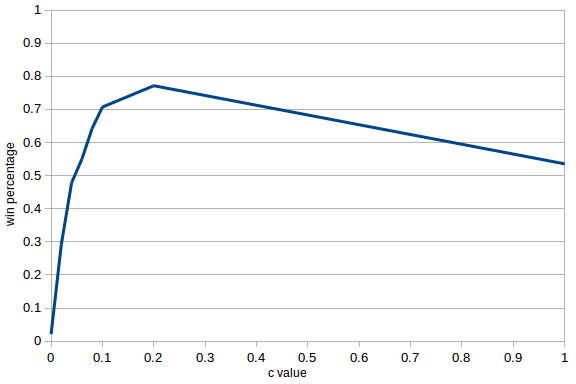
\includegraphics[width=\textwidth]{images/rank-0-01}
		\caption{Results of 8 c-values focused in the $[0,01]$ interval. Data can be found in appendix table \ref{table:ranking-matrix-random-zero}.}
		\label{fig:results-rank-0-01}
	\end{minipage}
\end{figure}

\section{How bad is a very low c-value}
Because a c-value of 0 showed a very bad result. I tested values close to 0 to test the behavior from 0 to 0.1. The population used was: \{0, 0.02, 0.04, 0.06, 0.08, 0.1, 0.2, 1\}. Figure \ref{fig:results-rank-0-01} shows performance increases rapidly from 0 to 0.2, at which point it decreases when going towards 1.0. This shows that the algorithm can exploit too much\footnote{Note a c-value of 0 is actually picking a random move, the algorithm will only look at one move and exploit it indefinitely}.

\begin{figure}[h]
	\centering
	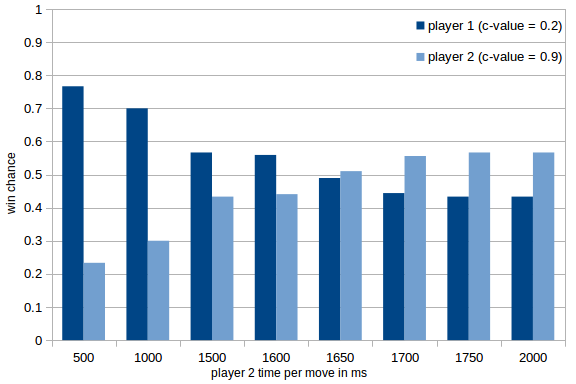
\includegraphics[width=0.5\textwidth]{images/mcts-significance}
	\caption{Win change between two players. Player 1 has c-value of 0.2 and 500ms per move. Player 2 has c-value of 0.9 and its time per move is on the x-axis. Each result is based on 30 games per result, except for the 1600, 1650 and 1700 results, those are based on 300 games. Data in appendix table \ref{table:impact-02-09}}
	\label{fig:mcts-significance}
\end{figure}
\section{What does a better c-value achieve}
As mentioned earlier, by using more time per move we can compensate for bad c-values. This allows us to actually measure the impact of a better performing c-value. I have tested how much more time worse c-values need to achieve similar performance as better c-values.\\
I've picked two different players, the first will have a c-value of 0.2 and 500ms per move. The second player has a c-value of 0.9 and will have its time per move changed until both players have about a 50\% win rate against each other. When both players have the same time per move (500ms) the win rate of the 0.2 player is 76.7\%\\
The win chance is based on 30 games. To reduce noise even further, for the 1600ms, 1650ms and 1700ms data points the win chances is based on $\sim300$ games. Figure \ref{fig:mcts-significance} shows 1650ms is very close to the 50\% mark. Indicating a player with c-value 0.9 needs $1650/500 = 3.3$ times as much time as a player with a c-value of 0.2 to get a 50\% win rate.\\


\textbf{TODO}
\begin{figure}[h]
	\centering
	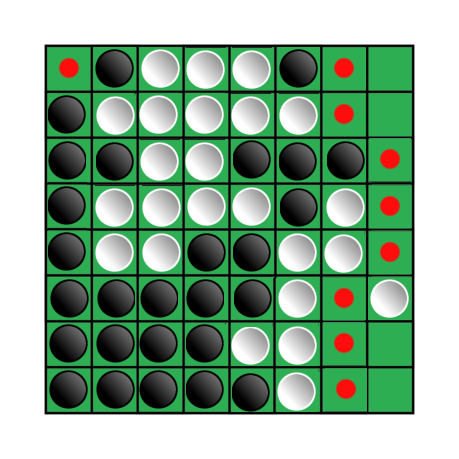
\includegraphics[width=0.25\textwidth]{images/corner-board}
	\caption{Othello board which allows black to make a corner move and even more importantly if black does not take the corner move, white can in the next move. This makes the corner move by far the best move. The red dots are possible moves for black.}
	\label{fig:othello-corner-board}
\end{figure}
\section{How well does it pick up 'smart' moves}
In Othello, corner moves are generally always good moves to make. To test how well MCTS picks this up on different c-values we've used the board in figure \ref{fig:othello-corner-board}. This board allows black to make a move.\\
\textbf{TODO}

\chapter{Conclusion}
In this paper I have sought to answer how important it is to use an optimal c-value for UCT. The results show a good c-value can have a significant positive impact, but finding such values might be very costly depending on specific use-cases. Ignoring the cost, finding these optimal c-values prove to be very helpful.\\

Several research questions have been stated to help answer the main question:
\begin{itemize}
	\setlength\itemsep{0em}
	\item How do different $c$-values for UCT compare?
	\item Is there any optimal $c$-value for a given problem?
	\item Is there a significant difference when using the optimal $c$-value versus other $c$-values?
\end{itemize}

The experiments showed when comparing different c-values, a very distinct pattern arose. In the specific problem of playing Othello optimal c-values are around the 0.18-0.23 range. With performance gradually sloping down for higher and lower values.\\
Even for reasonable close c-values, significant differences in performance have been shown. Multiple factors of extra time for UCT are needed when having to compensate for these differences in performance. Tuning the c-value can be very time consuming, therefor it might not always be worth to spend the time to find an optimal c-value. 


\textbf{TODO }- Terug loopen naar hoofdvraag + antwoord





\printbibliography

\centering
\begin{appendices}
\chapter{Experiment Data}
\section{Weighted simulation}

\begin{table}[H]
	\centering
	\begin{tabular}{|l|c|c|c|c|c|c|c|c|}
		\hline
		6.21 &  1.88 &  12.4 &  0.37 &  0.37 & 12.4  &  1.88 & 6.21 \\
		\hline
		1.88 & -1.00 & -5.45 & -1.40 & -1.40 & -5.45 & -1.00 & 1.88 \\
		\hline
		12.4 & -5.45 &  0.03 &  0.07 &  0.07 &  0.03 & -5.45 & 12.4 \\
		\hline
		0.37 & -1.40 &  0.07 & -1.32 & -1.32 &  0.07 & -1.40 & 0.37 \\
		\hline
		0.37 & -1.40 &  0.07 & -1.32 & -1.32 &  0.07 & -1.40 & 0.37 \\
		\hline
		12.4 & -5.45 &  0.03 &  0.07 &  0.07 &  0.03 & -5.45 & 12.4 \\
		\hline
		1.88 & -1.00 & -5.45 & -1.40 & -1.40 & -5.45 & -1.00 & 1.88 \\
		\hline
		6.21 &  1.88 & 12.4  &  0.37 &  0.37 & 12.4  &  1.88 & 6.21 \\
		\hline
	\end{tabular}
	\caption{Evolved weights for MCP(OC) from Experiments with Monte Carlo Othello\cite{hingston2007experiments}}
	\label{table:othello-weights}
\end{table}

\section{Raw data}
\begin{table}[H]
\[
\begin{array}{|c|c|}
    \hline
    \text{c-value} & \text{wins}\\
    \hline
	0.25 & 94 \\ 
	0.5 & 89 \\ 
	0.75 & 65 \\ 
	1 & 68 \\ 
	1.25 & 62 \\ 
	1.5 & 63 \\ 
	1.75 & 61 \\ 
	2 & 58 \\
	\hline
\end{array} 
\]
\caption{Raw data for a pool of c-values competing with each other.}
\label{table:results-rank-raw}
\end{table}

\section{Game results for different simulation types}

\subsection{Graph}
\begin{figure}[H]
	\centering
	\includegraphics[width=1\textwidth]{images/rank-015-3-sims}
	\caption{Same test as \ref{fig:results-rank-015} but with 3 seperate domain knowledge implementations. Raw data below.}
\end{figure}

\subsection{Random simulation}
\begin{table}[H]
	\centering
	\begin{tabular}{|l||l|l|l|l|l|l|l|l|l|l|l|l|l|}
		\hline
		& 0.0 & 0.1 & 0.2 & 0.3 & 0.4 & 0.5 & 0.6 & 0.7 & 0.8 & 0.9 & 1.0 & 3.0 & 5.0 \\ \hline
	    \hline
		0.0 & -   & 0   & 0   & 0   & 0   & 0   & 0   & 0   & 0   & 0   & 0   & 0   & 0   \\ \hline
		0.1 & 20  & -   & 8   & 6   & 9   & 8   & 9   & 12  & 14  & 15  & 11  & 14  & 15  \\ \hline
		0.2 & 20  & 12  & -   & 14  & 12  & 11  & 11  & 12  & 11  & 12  & 15  & 14  & 18  \\ \hline
		0.3 & 20  & 14  & 6   & -   & 12  & 11  & 11  & 11  & 12  & 14  & 13  & 19  & 16  \\ \hline
		0.4 & 20  & 11  & 8   & 8   & -   & 13  & 11  & 12  & 10  & 12  & 14  & 14  & 15  \\ \hline
		0.5 & 20  & 12  & 9   & 9   & 7   & -   & 9   & 10  & 12  & 12  & 9   & 14  & 17  \\ \hline
		0.6 & 20  & 11  & 9   & 9   & 9   & 11  & -   & 12  & 12  & 9   & 12  & 11  & 12  \\ \hline
		0.7 & 20  & 8   & 8   & 9   & 8   & 10  & 8   & -   & 8   & 11  & 12  & 14  & 14  \\ \hline
		0.8 & 20  & 6   & 9   & 8   & 10  & 8   & 8   & 12  & -   & 8   & 10  & 10  & 12  \\ \hline
		0.9 & 20  & 5   & 8   & 6   & 8   & 8   & 11  & 9   & 12  & -   & 10  & 8   & 11  \\ \hline
		1.0 & 20  & 9   & 5   & 7   & 6   & 11  & 8   & 8   & 10  & 10  & -   & 10  & 10  \\ \hline
		3.0 & 20  & 6   & 6   & 1   & 6   & 6   & 9   & 6   & 10  & 12  & 10  & -   & 11  \\ \hline
		5.0 & 20  & 5   & 2   & 4   & 5   & 3   & 8   & 6   & 8   & 9   & 10  & 9   & -   \\ \hline
	\end{tabular}
	\caption{Game results - 13 c-values each played 240 times versus a different c-value using random simulation. Each cell shows how many times the c-value on the y-axis won out of 20 possible games. Note that the matrix is diagonally mirrored, making cell a,b + b,c = 20}
	\label{table:ranking-matrix-random}
\end{table}

\subsection{Corners simulation}
\begin{table}[H]
	\centering
	\begin{tabular}{|l||l|l|l|l|l|l|l|l|l|l|l|l|l|}
		\hline 
		& 0.0 & 0.1 & 0.2 & 0.3 & 0.4 & 0.5 & 0.6 & 0.7 & 0.8 & 0.9 & 1.0 & 3.0 & 5.0 \\ \hline
		\hline
		0.0 & -   & 0   & 0   & 0   & 0   & 0   & 0   & 0   & 0   & 0   & 0   & 0   & 0   \\ \hline
		0.1 & 20  & -   & 8   & 15  & 8   & 15  & 11  & 17  & 15  & 15  & 11  & 16  & 18  \\ \hline
		0.2 & 20  & 12  & -   & 14  & 10  & 10  & 15  & 18  & 17  & 18  & 17  & 15  & 18  \\ \hline
		0.3 & 20  & 5   & 6   & -   & 12  & 8   & 12  & 13  & 15  & 14  & 16  & 14  & 18  \\ \hline
		0.4 & 20  & 12  & 10  & 8   & -   & 10  & 8   & 11  & 10  & 9   & 14  & 12  & 16  \\ \hline
		0.5 & 20  & 5   & 10  & 12  & 10  & -   & 9   & 9   & 9   & 15  & 12  & 14  & 14  \\ \hline
		0.6 & 20  & 9   & 5   & 8   & 12  & 11  & -   & 13  & 9   & 11  & 12  & 12  & 14  \\ \hline
		0.7 & 20  & 3   & 2   & 7   & 9   & 11  & 7   & -   & 11  & 13  & 11  & 15  & 15  \\ \hline
		0.8 & 20  & 5   & 3   & 5   & 10  & 11  & 11  & 9   & -   & 8   & 11  & 13  & 11  \\ \hline
		0.9 & 20  & 5   & 2   & 6   & 11  & 5   & 9   & 7   & 12  & -   & 13  & 14  & 13  \\ \hline
		1.0 & 20  & 9   & 3   & 4   & 6   & 8   & 8   & 9   & 9   & 7   & -   & 13  & 11  \\ \hline
		3.0 & 20  & 4   & 5   & 6   & 8   & 6   & 8   & 5   & 7   & 6   & 7   & -   & 10  \\ \hline
		5.0 & 20  & 2   & 2   & 2   & 4   & 6   & 6   & 5   & 9   & 7   & 9   & 10  & -   \\ \hline
	\end{tabular}
	\caption{Game results Corners - 13 c-values each played 240 times versus a different c-value using corners simulation. Each cell shows how many times the c-value on the y-axis won versus the c-value on the x-axis out of 20 possible games. Note that the matrix is diagonally mirrored, making cell a,b + b,c = 20}
	\label{table:ranking-matrix-corners}
\end{table}


\newcommand{\ifequals}[3]{\ifthenelse{\equal{#1}{#2}}{#3}{}}
\newcommand{\case}[2]{#1 #2} % Dummy, so \renewcommand has something to overwrite...
\newenvironment{switch}[1]{\renewcommand{\case}{\ifequals{#1}}}{}

\newcommand{\PercentRed}[1]{
	\ifnum #1<9
	1
	\else
	\ifnum #1 < 12
	0.9
	\else
	0.2
	\fi
	\fi
}

\newcommand{\PercentGreen}[1]{
	\ifnum #1<9
	0.2
	\else
	\ifnum #1 < 12
	0.9
	\else
	1
	\fi
	\fi
}

\newcommand{\PercentBlue}[1]{
	\ifnum #1<9
	0.2
	\else
	\ifnum #1 < 12
	0
	\else
	0.2
	\fi
	\fi
}

\newcommand{\ApplyGradient}[1] {
	\IfSubStr{#1}{-}{
		#1
	}{%
	\IfSubStr{#1}{.}{#1}{
		\cellcolor[rgb]{\PercentRed{#1},\PercentGreen{#1}, \PercentBlue{#1}}#1
	}
}%
}

\newcolumntype{R}{>{\collectcell\ApplyGradient}c<{\endcollectcell}}


\subsection{Weighted simulation}
\begin{table}[H]	
	\centering
	\begin{tabular}{|l||R|R|R|R|R|R|R|R|R|R|R|R|R|}
		\hline
		& 0.0 & 0.1 & 0.2 & 0.3 & 0.4 & 0.5 & 0.6 & 0.7 & 0.8 & 0.9 & 1.0 & 3.0 & 5.0 \\ \hline
		\hline
		0.0 & -   & 0   & 0   & 0   & 2   & 0   & 0   & 0   & 0   & 0   & 0   & 0   & 0   \\ \hline
		0.1 & 20  & -   & 10  & 11  & 8   & 10  & 14  & 17  & 10  & 11  & 12  & 19  & 17  \\ \hline
		0.2 & 20  & 10  & -   & 9   & 12  & 13  & 14  & 13  & 11  & 12  & 12  & 17  & 17  \\ \hline
		0.3 & 20  & 9   & 11  & -   & 8   & 13  & 11  & 16  & 13  & 11  & 15  & 18  & 13  \\ \hline
		0.4 & 18  & 12  & 8   & 12  & -   & 15  & 11  & 13  & 11  & 15  & 14  & 15  & 16  \\ \hline
		0.5 & 20  & 10  & 7   & 7   & 5   & -   & 12  & 14  & 14  & 13  & 12  & 14  & 15  \\ \hline
		0.6 & 20  & 6   & 6   & 9   & 9   & 8   & -   & 11  & 15  & 11  & 10  & 14  & 14  \\ \hline
		0.7 & 20  & 3   & 7   & 4   & 7   & 6   & 9   & -   & 9   & 8   & 13  & 7   & 8   \\ \hline
		0.8 & 20  & 10  & 9   & 7   & 9   & 6   & 5   & 11  & -   & 12  & 7   & 13  & 13  \\ \hline
		0.9 & 20  & 9   & 8   & 9   & 5   & 7   & 9   & 12  & 8   & -   & 8   & 11  & 10  \\ \hline
		1.0 & 20  & 8   & 8   & 5   & 6   & 8   & 10  & 7   & 13  & 12  & -   & 11  & 10  \\ \hline
		3.0 & 20  & 1   & 3   & 2   & 5   & 6   & 6   & 13  & 7   & 9   & 9   & -   & 11  \\ \hline
		5.0 & 20  & 3   & 3   & 7   & 4   & 5   & 6   & 12  & 7   & 10  & 10  & 9   & -   \\ \hline
	\end{tabular}
	\caption{Game results - 13 c-values each played 240 times versus a different c-value using weighted simulation. Each cell shows how many times the c-value on the y-axis won out of 20 possible games. Note that the matrix is diagonally mirrored, making cell a,b + b,c = 20}
	\label{table:ranking-matrix-weighted}
\end{table}

\section{[0.18,0.24] interval}
\begin{table}[H]
	\centering
	\begin{tabular}{|l||l|l|l|l|l|l|l|}
		\hline
		     & 0.18 & 0.19 & 0.2 & 0.21 & 0.22 & 0.23 & 0.24    \\ \hline \hline
		0.18 & -    & 9   & 12   & 12   & 8    & 11   & 10 \\ \hline
		0.19 & 11   & -   & 9    & 14   & 13   & 14   & 9  \\ \hline
		0.2  & 8    & 11  & -    & 11   & 9    & 7    & 11 \\ \hline
		0.21 & 8    & 6   & 9    & -    & 12   & 6    & 13 \\ \hline
		0.22 & 12   & 7   & 11   & 8    & -    & 10   & 8  \\ \hline
		0.23 & 9    & 6   & 13   & 14   & 10   & -    & 10 \\ \hline
		0.24 & 10   & 11  & 9    & 7    & 12   & 10   & -  \\ \hline
	\end{tabular}
		\caption{Game results Random - 7 c-values compete concentrated in the 0.18 - 0.24 interval. Each cell shows how many times the c-value on the y-axis won versus the c-value on the x-axis out of 20 possible games. Note that the matrix is diagonally mirrored, making cell a,b + b,c = 20 games.}
		\label{table:ranking-matrix-random-narrow}
\end{table}

\section{[1.18, 1.24] interval}
\begin{table}[H]
	\centering
	\begin{tabular}{|l||l|l|l|l|}
		\hline
		& 1.18 & 1.2 & 1.22 & 1.24 \\ \hline\hline
		1.18 & -     & 10  & 8    & 9    \\ \hline
		1.2  & 10   & -   & 7    & 9    \\ \hline
		1.22 & 12   & 13  & -    & 10   \\ \hline
		1.24 & 11   & 11  & 10   & -    \\ \hline
	\end{tabular}
	\caption{Game results Random - 4 c-values compete concentrated in the 1.18 - 1.24 interval. Each cell shows how many times the c-value on the y-axis won versus the c-value on the x-axis out of 20 possible games. Note that the matrix is diagonally mirrored, making cell a,b + b,c = 20 games.}
	\label{table:ranking-matrix-random-narrow2}
\end{table}


\section{[0,0.1] interval}
\begin{table}[H]
	\centering
	\begin{tabular}{|l||l|l|l|l|l|l|l|l|}
		\hline
		& 0.0 & 0.02 & 0.04 & 0.06 & 0.08 & 0.1 & 0.2 & 1.0 \\ \hline\hline
		0.0  & -   & 2    & 1    & 0    & 0    & 0   & 0   & 0   \\ \hline
		0.02 & 18  & -    & 6    & 5    & 2    & 3   & 1   & 6   \\ \hline
		0.04 & 19  & 14   & -    & 9    & 8    & 6   & 4   & 7   \\ \hline
		0.06 & 20  & 15   & 11   & -    & 6    & 7   & 5   & 13  \\ \hline
		0.08 & 20  & 18   & 12   & 14   & -    & 8   & 9   & 9   \\ \hline
		0.1  & 20  & 17   & 14   & 13   & 12   & -   & 8   & 15  \\ \hline
		0.2  & 20  & 19   & 16   & 15   & 11   & 12  & -   & 15  \\ \hline
		1.0  & 20  & 14   & 13   & 7    & 11   & 5   & 5   & -   \\ \hline
	\end{tabular}
	\caption{Game results random simulation - 8 c-values each played 140 times versus a different c-value using corners simulation. Each cell shows how many times the c-value on the y-axis won versus the c-value on the x-axis out of 20 possible games. Note that the matrix is diagonally mirrored, making cell a,b + b,c = 20}
	\label{table:ranking-matrix-random-zero}
\end{table}

\section{C-value impact}
\begin{table}[H]
	\begin{tabular}{|l||l|l|l|l|}
		\hline
		Ai 2 time & Games played & Ai 1 games won & Ai 2 games won & Ai 1 win \% \\ \hline \hline
		500       & 28           & 21             & 9              & 76.7\%      \\ \hline
		1000      & 30           & 21             & 9              & 70.0\%      \\ \hline
		1500      & 30           & 17             & 13             & 56.7\%      \\ \hline
		1600      & 490          & 274            & 216            & 55.9\%      \\ \hline
		1650      & 388          & 190            & 198            & 48.9\%      \\ \hline
		1700      & 232          & 103            & 129            & 44.3\%      \\ \hline
		1750      & 30           & 13             & 17             & 43.3\%      \\ \hline
		2000      & 30           & 13             & 17             & 43.3\%      \\ \hline
	\end{tabular}
	\centering
	\caption{Game data for 2 ai players. AI player 1 had c-value of 0.2 and 500ms per move. AI player 2 had c-value of 0.9 and increasing time per move (column 1)}
	\label{table:impact-02-09}
\end{table}

\end{appendices}

\end{document}
